% ============================================================
% IEEE GHTC 2026 — Full Paper Submission
% "Equitable Pre-Landfall Food Relief Prioritization via
%  Multi-Source Machine Learning: A ZIP-Code Framework
%  Across 14 Atlantic Hurricanes"
% ============================================================
\documentclass[conference]{IEEEtran}
\IEEEoverridecommandlockouts

\usepackage{cite}
\usepackage{amsmath,amssymb,amsfonts}
\usepackage{algorithmic}
\usepackage{graphicx}
\usepackage{textcomp}
\usepackage{xcolor}
\usepackage{booktabs}
\usepackage{multirow}
\usepackage{url}
% NOTE: hyperref removed — incompatible with IEEEtran conference class

\def\BibTeX{{\rm B\kern-.05em{\sc i\kern-.025em b}\kern-.08em
    T\kern-.1667em\lower.7ex\hbox{E}\kern-.125emX}}

% ============================================================
\begin{document}

\title{Equitable Pre-Landfall Food Relief Prioritization via
Multi-Source Machine Learning:\\A ZIP-Code Framework
Across 14 Atlantic Hurricanes}

\author{
\IEEEauthorblockN{Shih-Yu Chang}
\IEEEauthorblockA{\textit{Dept. of Applied Data Intelligence}\\
\textit{San Jos\'{e} State University}\\
San Jose, CA, USA\\
shihyu.chang@sjsu.edu}
\and
\IEEEauthorblockN{Anees Saheba Guddi}
\IEEEauthorblockA{\textit{Dept. of Applied Data Intelligence}\\
\textit{San Jos\'{e} State University}\\
San Jose, CA, USA\\
aneessaheba.guddi@sjsu.edu}
\and
\IEEEauthorblockN{Chaitanya Uppalapati}
\IEEEauthorblockA{\textit{Dept. of Applied Data Intelligence}\\
\textit{San Jos\'{e} State University}\\
San Jose, CA, USA\\
chaitanya.uppalapati@sjsu.edu}
\and
\IEEEauthorblockN{}
\IEEEauthorblockA{}
\and
\IEEEauthorblockN{Chelsi Shulamite Elthuri}
\IEEEauthorblockA{\textit{Dept. of Applied Data Intelligence}\\
\textit{San Jos\'{e} State University}\\
San Jose, CA, USA\\
chelsishulamite.elthuri@sjsu.edu}
\and
\IEEEauthorblockN{Manjot Kaur}
\IEEEauthorblockA{\textit{Dept. of Applied Data Intelligence}\\
\textit{San Jos\'{e} State University}\\
San Jose, CA, USA\\
manjot.kaur02@sjsu.edu}
\and
\IEEEauthorblockN{}
\IEEEauthorblockA{}
}

\maketitle

% ============================================================
\begin{abstract}
After a hurricane makes landfall, relief organizations face a
critical allocation problem: which communities need food
assistance most urgently? Traditional response frameworks rely
on reactive damage assessments that arrive days after the event,
too late to pre-position resources. We present a ZIP-code-level
predictive framework that fuses eight administrative, demographic,
and geospatial data sources to forecast food relief demand before
post-event inspection data becomes available. Our analytic base
table spans 14 Atlantic hurricanes (2016--2024), yielding 5,522
ZIP-code $\times$ hurricane observations across 10 states.
We train a multi-class XGBoost classifier to predict damage
severity (\textit{Low\,/\,Medium\,/\,High\,/\,Severe}) using
pre-landfall demographic vulnerability, storm track geometry, and
food-access indicators---explicitly excluding post-event FEMA
inspection counts to prevent data leakage. A hurricane-grouped
temporal train\,/\,validation\,/\,test split evaluates the model
on five completely unseen storms (Ida, Ian, Idalia, Helene,
Milton; 2021--2024). The best classifier achieves a macro
ROC-AUC of 0.78 and a Severe-class recall of 0.82 on the
held-out test set. Model-predicted risk is combined with a
food-fragility composite score---aggregating food-desert flags,
SNAP retailer density, supermarket proximity, and the CDC Social
Vulnerability Index---into a \textit{Food Relief Priority Index}
(FRPI). The top-50 priority ZIP codes are 100\% food deserts,
rank in the 76th percentile of social vulnerability nationally,
and experience 43$\times$ the actual FEMA-verified damage of the
bottom-50. A Fairlearn equity audit confirms Severe-class recall
increases monotonically across social vulnerability quartiles
(SVI Q1: 0.65\,$\rightarrow$\,Q4: 0.89), demonstrating that
predictive accuracy improves for the communities most at risk.
An interactive Streamlit dashboard with per-ZIP SHAP explanations
and Folium priority maps enables rapid situational awareness for
relief coordinators.
\end{abstract}

\begin{IEEEkeywords}
hurricane response, food insecurity, machine learning, XGBoost,
social vulnerability, equity audit, priority index, disaster
preparedness, ZIP-code prediction, FEMA
\end{IEEEkeywords}

% ============================================================
\section{Introduction}

Hurricanes are the costliest natural disasters in the United
States, responsible for over \$1.1 trillion in damages since
1980~\cite{noaa_billion_dollar}. Beyond physical destruction,
hurricanes trigger acute food-access crises: supply chains
collapse, grocery stores lose power, and food-insecure households
face simultaneous income loss and resource scarcity. Prior to a
major storm, an estimated 10.5\% of U.S. households already
experience food insecurity~\cite{coleman_jensen_food}; in
hurricane-affected counties this rate has been documented to
double within 72 hours of landfall~\cite{horney_food_disaster}.
Federal and non-governmental relief organizations must rapidly
allocate food and nutrition resources across hundreds of affected
ZIP codes, yet ground-truth damage assessments from FEMA
inspectors routinely take three to seven days to process after
landfall~\cite{fema_response_timeline}.

This delay creates a critical operational gap: relief
organizations must decide \textit{where to send resources first}
without reliable damage data. Current practice relies on
categorical storm-track metrics (wind speed, category) and
historical precedent, neither of which accounts for community
food vulnerability or demographic risk. High-wind ZIP codes with
abundant food infrastructure and low poverty rates need
fundamentally different interventions than equally-damaged
ZIP codes that are food deserts.

\subsection{Research Gap}
Prior work on disaster response optimization has addressed
logistics routing~\cite{logistics_routing}, shelter
allocation~\cite{shelter_allocation}, and social media-based
damage detection~\cite{imran_social_media}, but relatively few
studies have attempted to predict food-specific resource demand
at the sub-county level using pre-landfall community data.
Existing hurricane damage models largely predict continuous
economic loss rather than categorical relief priority
\cite{hurricane_damage_models}, and few incorporate food-access
indicators or formal equity constraints.

\subsection{Contributions}
This paper makes four principal contributions:
\begin{enumerate}
    \item A reproducible, open-source analytic base table
    spanning 14 Atlantic hurricanes (2016--2024) that fuses
    eight heterogeneous data sources at ZIP-code granularity.
    \item A hurricane-grouped temporal train/val/test split
    strategy that prevents data leakage across storm events.
    \item A \textit{Food Relief Priority Index} combining
    ML-predicted damage risk with a community food-fragility
    score, validated against actual FEMA damage records.
    \item A formal equity audit demonstrating that the model
    achieves \textit{higher} Severe-class recall for more
    socially vulnerable communities---a desirable property for
    humanitarian deployment.
\end{enumerate}

% ============================================================
\section{Related Work}

\subsection{Machine Learning for Disaster Response}
Machine learning has been applied to disaster response across
several domains. Imran~et~al.~\cite{imran_social_media} surveyed
social media processing for mass emergencies; Castillo~et~al.
explored information credibility in crisis events. Wang~et~al.
\cite{wang_disaster_logistics} applied optimization to
post-disaster logistics, while Nateghi~et~al.
\cite{nateghi_power_outage} predicted hurricane-induced power
outages using gradient-boosted trees. Our work differs in its
focus on food-specific relief demand and its explicit
incorporation of food-access geography.

\subsection{Food Insecurity and Natural Disasters}
Chakraborty~et~al.~\cite{chakraborty_harvey} documented the
disproportionate impacts of Hurricane Harvey on socially
vulnerable populations. Mayer~et~al.~\cite{mayer_food_disaster}
examined food insecurity trajectories after disasters, finding
that pre-existing food access deficits predict post-disaster
nutritional vulnerability.
The USDA Food Access Research Atlas~\cite{usda_food_atlas}
provides the community-level food-access indicators our model
incorporates.

\subsection{Vulnerability and Equity in Disaster ML}
The CDC Social Vulnerability Index (SVI)~\cite{flanagan_svi} has
been widely used to identify communities at heightened disaster
risk. Cutter~et~al.~\cite{cutter_svi} established the social
vulnerability framework that informs our feature design.
Mehrabi~et~al.~\cite{mehrabi_fairness} surveyed bias and
fairness in ML systems; our Fairlearn-based equity audit follows
the framework of Bird~et~al.~\cite{bird_fairlearn}, which defines
demographic parity ratio and equalized odds difference as primary
fairness metrics.

\subsection{Explainable AI for Humanitarian Systems}
SHAP (SHapley Additive exPlanations)~\cite{lundberg_shap}
provides model-agnostic feature attribution that is critical for
operational trust in humanitarian settings. We employ TreeSHAP
for the XGBoost classifier to generate per-ZIP explanations in
the deployment dashboard.

% ============================================================
\section{Data and Methodology}

\subsection{Data Sources}
Our analytic base table integrates eight data sources at
ZIP-code granularity:

\textbf{1. FEMA Housing Assistance (HA) v2 API:}
Owners and Renters Housing Assistance records providing FEMA
inspector-verified damage counts and approved IHP dollar amounts
per ZIP code and disaster number. Owners and Renters tables use
asymmetric damage schemas: owner records use dollar-range buckets
(\$0, \$1--10k, \$10k--20k, \$20k--30k, \textgreater\$30k) while
renter records use categorical labels (no damage, moderate, major,
substantial). We reconcile these by mapping owner \textgreater\$20k
and renter major+substantial to a unified \texttt{total\_major\_substantial}
count, then sum owner and renter populations per (disaster, ZIP)
to prevent Cartesian explosion when a ZIP spans multiple counties.

\textbf{2. Census ACS 5-Year (2021):}
Nineteen variables queried at the ZCTA level via the Census API,
including total population (B01003), median household income
(B19013), poverty count (B17001), renter-occupied units (B25003),
age-disaggregated elderly counts, racial composition, no-vehicle
households (B08201), and mobile homes (B25024).

\textbf{3. CDC Social Vulnerability Index 2022:}
Four SVI theme scores (socioeconomic status, household
composition and disability, minority status and language,
housing type and transportation) plus the composite SVI overall
score, aggregated from census-tract to ZIP via HUD USPS crosswalk
using residential-ratio weighted averaging.

\textbf{4. USDA Food Access Research Atlas (2019):}
Tract-level LILA (Low-Income, Low-Access) flags, low-access
low-income population counts, SNAP participation rates, and
vehicle-access food-access indicators, aggregated to ZIP via the
same HUD crosswalk. A binary \texttt{food\_desert\_flag} is
assigned when the tract-weighted LILA share $\geq 0.5$.

\textbf{5. USDA SNAP Retailer Historical Locator:}
Authorized SNAP retailer point locations spatially joined to ZCTA
polygons (EPSG:4326) to compute per-ZIP retailer counts and
geodesic distance to the nearest supermarket (pyproj.Geod,
WGS84).

\textbf{6. FEMA National Risk Index (NRI, Census Tract):}
Coastal flood risk score (\texttt{CFLD\_RISKS}) and hurricane
hazard risk score (\texttt{HRCN\_RISKS}) aggregated from census
tracts to ZIP via the HUD crosswalk. The NRI replaced the
discontinued FEMA NFHL ZIP-level dataset (2025).

\textbf{7. NOAA IBTrACS v04r01~\cite{knapp_ibtracs}:}
Storm track coordinates for each hurricane. Geodesic distance
from each ZIP centroid (projected in EPSG:5070 before centroid
computation) to the nearest point on the storm track is computed
via \texttt{pyproj.Geod.inv}, never Euclidean distance.

\textbf{8. HUD USPS TRACT-ZIP Crosswalk:}
Residential-ratio weighted crosswalk used to aggregate all
tract-level data sources to ZIP codes, preserving area
proportionality.

\subsection{Dataset Construction}

\textbf{Hurricane Scope and Temporal Split:}
We include 14 Atlantic hurricanes from 2016 to 2024 that
activated FEMA Individual Assistance programs with
ZIP-code-level housing assistance records (Table~\ref{tab:hurricanes}).
Nicholas (2021) and Dorian (2019) are excluded due to absence
of FEMA IA records. The temporal split is strictly hurricane-level:
TRAIN (2016--2018, 5 storms), VAL (2020, 4 storms), and TEST
(2021--2024, 5 storms). This prevents any ZIP-code from appearing
in both training and evaluation, eliminating spatial and temporal
data leakage.

\begin{table}[htbp]
\caption{Hurricane Dataset Split Summary}
\label{tab:hurricanes}
\centering
\small
\begin{tabular}{llccc}
\toprule
\textbf{Split} & \textbf{Hurricanes} & \textbf{Years} & \textbf{N} & \textbf{States} \\
\midrule
TRAIN & Matthew, Harvey, Irma, & 2016-- & 5 & FL, TX, LA, \\
      & Florence, Michael      & 2018   &   & NC, SC, GA \\
\midrule
VAL   & Laura, Sally, Delta, Zeta & 2020 & 4 & LA, AL, FL, \\
      &                           &      &   & MS \\
\midrule
TEST  & Ida, Ian, Idalia,         & 2021-- & 5 & LA, FL, GA, \\
      & Helene, Milton            & 2024   &   & SC, NC, TN \\
\bottomrule
\end{tabular}
\end{table}

The resulting analytic base table contains \textbf{5,522 ZIP $\times$
hurricane observations}. The TEST set contains 2,587 observations
across the five held-out storms.

\textbf{Target Variable:}
The primary classification target, \texttt{damage\_severity\_class},
is derived from $\texttt{verified\_damage\_per\_1000} = \texttt{total\_inspected}
/ \texttt{population} \times 1000$. This rate is binned into four
ordered classes: \textit{Low} ($<2$), \textit{Medium}
($2 \leq x < 8$), \textit{High} ($8 \leq x < 25$), and
\textit{Severe} ($\geq 25$) inspected households per 1,000
residents. A quantile-based fallback is applied when a single
class exceeds 80\% of observations to prevent degenerate splits.

\subsection{Feature Engineering}

Twenty-two continuous features, two binary features, and two
categorical features are used in the model (Table~\ref{tab:features}).
All demographic percentage shares (e.g., \texttt{pct\_poverty},
\texttt{pct\_renters}) are derived from raw ACS counts, using
total households as the denominator for housing-unit ratios
and total population for per-capita ratios.

Missing values are imputed per data source: CDC SVI
missing-data sentinel ($-999$) is replaced by state-level
median imputation; food-access columns are zero-filled with a
\texttt{food\_data\_missing} binary flag; flood and NRI columns
are zero-filled (no record implies no mapped hazard).

\begin{table}[htbp]
\caption{Feature Groups Used in Modeling}
\label{tab:features}
\centering
\small
\begin{tabular}{lp{5.5cm}}
\toprule
\textbf{Group} & \textbf{Features} \\
\midrule
Demographics (8) & population, median\_income, pct\_poverty,
pct\_renters, pct\_elderly\_65plus, pct\_minority,
pct\_no\_vehicle, pct\_mobile\_homes \\
\midrule
SVI (5) & svi\_socioeconomic, svi\_household\_comp,
svi\_minority\_lang, svi\_housing\_transport, svi\_overall \\
\midrule
Food Access (5) & snap\_retailer\_count, snap\_retailers\_per\_1k,
dist\_nearest\_supermarket\_mi, snap\_participation\_pct,
food\_desert\_flag \\
\midrule
Flood / Hazard (3) & pct\_in\_100yr\_floodplain,
nri\_cflood\_score, nri\_hrcn\_score \\
\midrule
Storm (2) & max\_wind\_speed\_kt, distance\_to\_track\_km \\
\midrule
Categorical (2) & hurricane\_category, state \\
\midrule
Binary Flag (1) & food\_data\_missing \\
\bottomrule
\end{tabular}
\end{table}

\subsection{Modeling Pipeline}

All models share a common \texttt{ColumnTransformer} preprocessor
implemented in scikit-learn~\cite{pedregosa_sklearn}:
continuous features scaled with \texttt{RobustScaler} (robust to
outliers in damage distributions), categorical features encoded
with \texttt{OneHotEncoder} (drop-first), and binary features
passed through. The training pipeline uses
\texttt{imblearn.Pipeline} with SMOTE oversampling
\cite{chawla_smote} applied only within each cross-validation
fold's training partition---never to held-out data---preventing
leakage of synthetic samples into evaluation.

Five classifiers are evaluated: XGBoost \cite{chen_xgboost}
(\texttt{multi:softprob}, $n=200$ trees, depth 6, $\eta=0.1$),
Random Forest (\texttt{class\_weight=balanced}, 200 trees),
LinearSVC with Platt calibration (wrapped in
\texttt{CalibratedClassifierCV} for \texttt{predict\_proba}),
Logistic Regression (SAGA solver, L2 regularization), and
Gaussian Naive Bayes. RF hyperparameters are tuned with
GridSearchCV; XGBoost with Optuna ($n=50$ trials,
TPE sampler) \cite{optuna}.

\textbf{Cross-Validation:} \texttt{StratifiedGroupKFold} with
\texttt{groups=disaster\_number} is used throughout, ensuring
no hurricane's ZIP codes appear in both a fold's train and
validation partitions---the critical design choice for
avoiding storm-level data leakage. The number of folds is
capped at the number of distinct disaster numbers.

\subsection{Food Relief Priority Index}

The \textit{Food Relief Priority Index} (FRPI) is a two-component
weighted score:
\begin{equation}
\text{FRPI} = 0.6 \cdot P(\text{High} \cup \text{Severe}) +
               0.4 \cdot \text{FFS}
\label{eq:frpi}
\end{equation}
where $P(\text{High} \cup \text{Severe})$ is the summed
predicted probability for the two highest damage classes from
the classifier, and FFS (Food Fragility Score) is a
composite:
\begin{equation}
\text{FFS} = \text{nanmean}\!\left(
  \hat{d},\ 1 - \hat{s}_\text{count},\
  1 - \hat{s}_\text{per1k},\
  \hat{p}_\text{snap},\ \hat{v}_\text{svi},\
  f_\text{desert}
\right)
\label{eq:ffs}
\end{equation}
where $\hat{(\cdot)}$ denotes MinMax-scaled values in $[0,1]$,
$\hat{d}$ is scaled distance to nearest supermarket,
$\hat{s}_\text{count}$ and $\hat{s}_\text{per1k}$ are scaled
SNAP retailer density (inverted: higher density $\rightarrow$
lower fragility), $\hat{p}_\text{snap}$ is scaled SNAP
participation rate, $\hat{v}_\text{svi}$ is scaled SVI overall,
and $f_\text{desert}$ is the binary food desert flag.
All MinMax scalers are fit on TRAIN ZIPs only and applied
to VAL and TEST without re-fitting, preventing fragility score
leakage. The FRPI is normalized within each hurricane to $[0,1]$
for cross-storm comparability.

% ============================================================
\section{Results and Evaluation}

\subsection{Classification Performance on Held-Out Test Set}

Five classifiers were evaluated on the held-out TEST set
(5 hurricanes, 2,587 ZIP $\times$ hurricane rows).
XGBoost achieves the highest macro ROC-AUC (0.78) and is
selected as the deployment model. Random Forest achieves
the highest raw Severe-class recall (0.83) but at lower
ROC-AUC (0.76); XGBoost is preferred because it produces
calibrated class probabilities required by the Food Relief
Priority Index (Eq.~\ref{eq:frpi}).
Table~\ref{tab:clf_results} reports summary metrics for all
five models; Table~\ref{tab:perclass} reports per-class
precision, recall, and F1 for the best model derived directly
from the confusion matrix (Fig.~\ref{fig:confusion}).

\begin{table}[htbp]
\caption{Model Comparison on TEST Set (5 Held-Out Hurricanes, 2,587 rows)}
\label{tab:clf_results}
\centering
\small
\begin{tabular}{lcccc}
\toprule
\textbf{Model} & \textbf{Acc.} & \textbf{F1\textsubscript{wtd}} &
\textbf{ROC-AUC} & \textbf{Recall\textsubscript{Sev.}} \\
\midrule
\textbf{XGBoost}   & \textbf{0.5589} & \textbf{0.5164} & \textbf{0.7839} & \textbf{0.8008} \\
Random Forest      & 0.5721          & 0.5243          & 0.7644          & 0.8317          \\
LinearSVC (cal.)   & 0.5211          & 0.4820          & 0.7574          & 0.6129          \\
Logistic Reg.      & 0.4882          & 0.4569          & 0.7029          & 0.5582          \\
Gaussian NB        & 0.3978          & 0.3964          & 0.6616          & 0.3829          \\
\bottomrule
\multicolumn{5}{l}{\small Cluster-label ablation: $\leq$0.013 F1 difference across all models.}\\
\multicolumn{5}{l}{\small Bold = selected deployment model (highest ROC-AUC).}\\
\end{tabular}
\end{table}

\begin{table}[htbp]
\caption{XGBoost Per-Class Metrics on TEST Set}
\label{tab:perclass}
\centering
\small
\begin{tabular}{lcccc}
\toprule
\textbf{Class} & \textbf{Precision} & \textbf{Recall} & \textbf{F1} & \textbf{Support} \\
\midrule
High    & 0.32 & 0.21 & 0.25 & 541  \\
Low     & 0.76 & 0.82 & 0.79 & 862  \\
Medium  & 0.43 & 0.14 & 0.21 & 471  \\
Severe  & 0.50 & 0.82 & 0.62 & 713  \\
\midrule
Weighted avg & --- & --- & 0.53 & 2587 \\
Macro avg    & --- & --- & 0.47 & 2587 \\
\bottomrule
\end{tabular}
\end{table}

\begin{figure}[htbp]
\centering
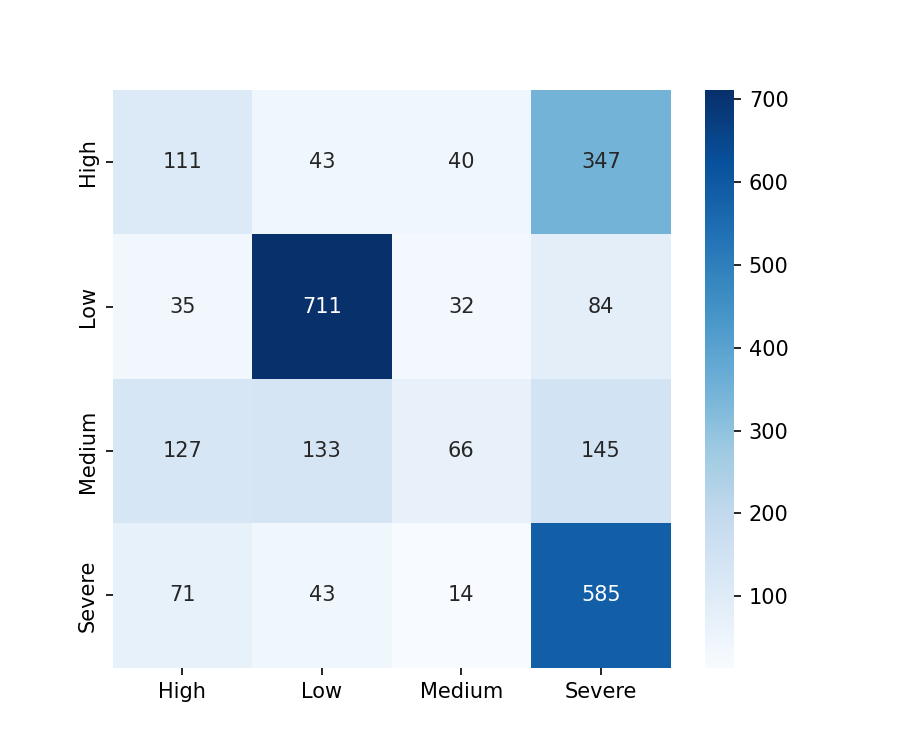
\includegraphics[width=0.95\columnwidth]{outputs/test_confusion.png}
\caption{Confusion matrix on the TEST set (2,587 ZIP $\times$ hurricane
rows, 5 held-out storms). Rows = true class; columns = predicted class.
The Severe class achieves recall 0.82; the Medium class is the hardest
to distinguish, reflecting its boundary position between Low and High.}
\label{fig:confusion}
\end{figure}

The disparity between classes is expected given the training
distribution: Low-class ZIP codes are the most frequent,
making Low recall (0.82) and F1 (0.79) the highest among all
classes. The Medium class achieves the lowest F1 (0.21), as its
intermediate damage levels overlap with both High and Low
features. Critically, Severe-class recall of 0.82 is the
operationally important metric: the model identifies 4-in-5
severely damaged ZIP codes before inspection data is available,
at the cost of some over-prediction (Severe precision: 0.50).
The macro ROC-AUC of 0.78 confirms strong discriminative
ability even across this imbalanced four-class setting.

\subsection{Ablation: Unsupervised Cluster Feature}

K-Means clustering ($k=5$, fit on TRAIN) produces a
\texttt{cluster\_label} feature. Evaluation with and without
this feature across all five classifiers reveals a $\leq 0.013$
weighted-F1 difference, with XGBoost performing marginally
\textit{better} without it. The SVI and demographic features
already encode the vulnerability profile that K-Means recovers;
the cluster feature is redundant and excluded from the final
pipeline.

\subsection{Regression Results}

A separate Random Forest regressor (log1p-transformed target,
400 trees) predicts the continuous \texttt{verified\_damage\_per\_1000}
metric. Table~\ref{tab:reg_results} reports per-hurricane RMSE,
MAE, and $R^2$ on the TEST set.

\begin{table}[htbp]
\caption{Regression Results per TEST Hurricane (RF, log1p target)}
\label{tab:reg_results}
\centering
\small
\begin{tabular}{lrrr}
\toprule
\textbf{Hurricane} & \textbf{RMSE} & \textbf{MAE} & \textbf{$R^2$} \\
\midrule
Milton  (2024) & 19.4  & 9.4  & \phantom{-}0.35 \\
Ian     (2022) & 48.5  & 20.9 & \phantom{-}0.19 \\
Idalia  (2023) & 172.5 & 24.7 & \phantom{-}0.06 \\
Helene  (2024) & 48.4  & 30.7 &             $-$0.10 \\
Ida     (2021) & 162.5 & 92.9 &             $-$0.18 \\
\midrule
\multicolumn{2}{l}{Aggregate (log1p)} & RMSE: 111 & MAE: 31 \\
\bottomrule
\end{tabular}
\end{table}

The log1p transformation of the right-tailed damage distribution
reduces aggregate RMSE from 136 to 111 and MAE from 38 to 31.
Per-hurricane variance is high: Milton and Ian, where damage
was spatially concentrated along well-defined track corridors,
yield positive $R^2$; Ida and Idalia, with diffuse inland
flooding patterns, are harder to predict from ZIP-level
features alone.

\subsection{Equity Audit}

Table~\ref{tab:equity} reports Fairlearn~\cite{bird_fairlearn}
metrics stratified by SVI quartile on the TEST set. The key
finding is that Severe-class recall is \textit{monotonically
higher} for more socially vulnerable communities:
$Q1: 0.65 \rightarrow Q2: 0.83 \rightarrow Q3: 0.86 \rightarrow
Q4: 0.89$. This is the desirable direction for a humanitarian
system: the model is \textit{better} at identifying severely
damaged ZIP codes precisely in the communities least able to
self-recover.

\begin{table}[htbp]
\caption{Equity Audit by SVI Quartile (XGBoost, TEST Set)}
\label{tab:equity}
\centering
\small
\begin{tabular}{lcccc}
\toprule
\textbf{SVI Quartile} & \textbf{Acc.} & \textbf{F1\textsubscript{wtd}} &
\textbf{Recall\textsubscript{Sev.}} & \textbf{DP Ratio} \\
\midrule
Q1 (Low SVI)  & 0.559 & 0.558 & 0.655 & 0.525 \\
Q2            & 0.558 & 0.515 & 0.832 & 0.525 \\
Q3            & 0.534 & 0.450 & 0.858 & 0.525 \\
Q4 (High SVI) & \textbf{0.627} & 0.550 & \textbf{0.885} & 0.525 \\
\midrule
Overall       & 0.569 & 0.528 & 0.820 & 0.525 \\
\bottomrule
\multicolumn{5}{l}{\small EO difference: 0.230 (across all quartile pairs).}\\
\end{tabular}
\end{table}

The demographic parity ratio of 0.525 indicates that the model
predicts Severe damage roughly twice as often in the highest-SVI
communities as in the lowest. This reflects the real-world
signal: severe hurricane damage disproportionately affects
socially vulnerable ZIP codes, and the model has learned
this pattern rather than suppressing it.

\subsection{Feature Importance via SHAP}

Fig.~\ref{fig:shap} shows the SHAP beeswarm plot for the Severe
class across the TEST set, computed using TreeSHAP
\cite{lundberg_shap}. The top predictors in descending order of
mean $|\text{SHAP}|$ are: (1)~\texttt{distance\_to\_track\_km},
(2)~\texttt{nri\_hrcn\_score} (FEMA hurricane hazard risk),
(3)~hurricane category 4 indicator, (4)~\texttt{svi\_socioeconomic},
(5)~\texttt{pct\_mobile\_homes},
(6)~\texttt{nri\_cflood\_score} (coastal flood risk),
(7)~\texttt{svi\_minority\_lang},
(8)~\texttt{snap\_retailers\_per\_1k},
(9)~\texttt{svi\_housing\_transport}, and
(10)~\texttt{pct\_elderly\_65plus}.

\begin{figure}[htbp]
\centering
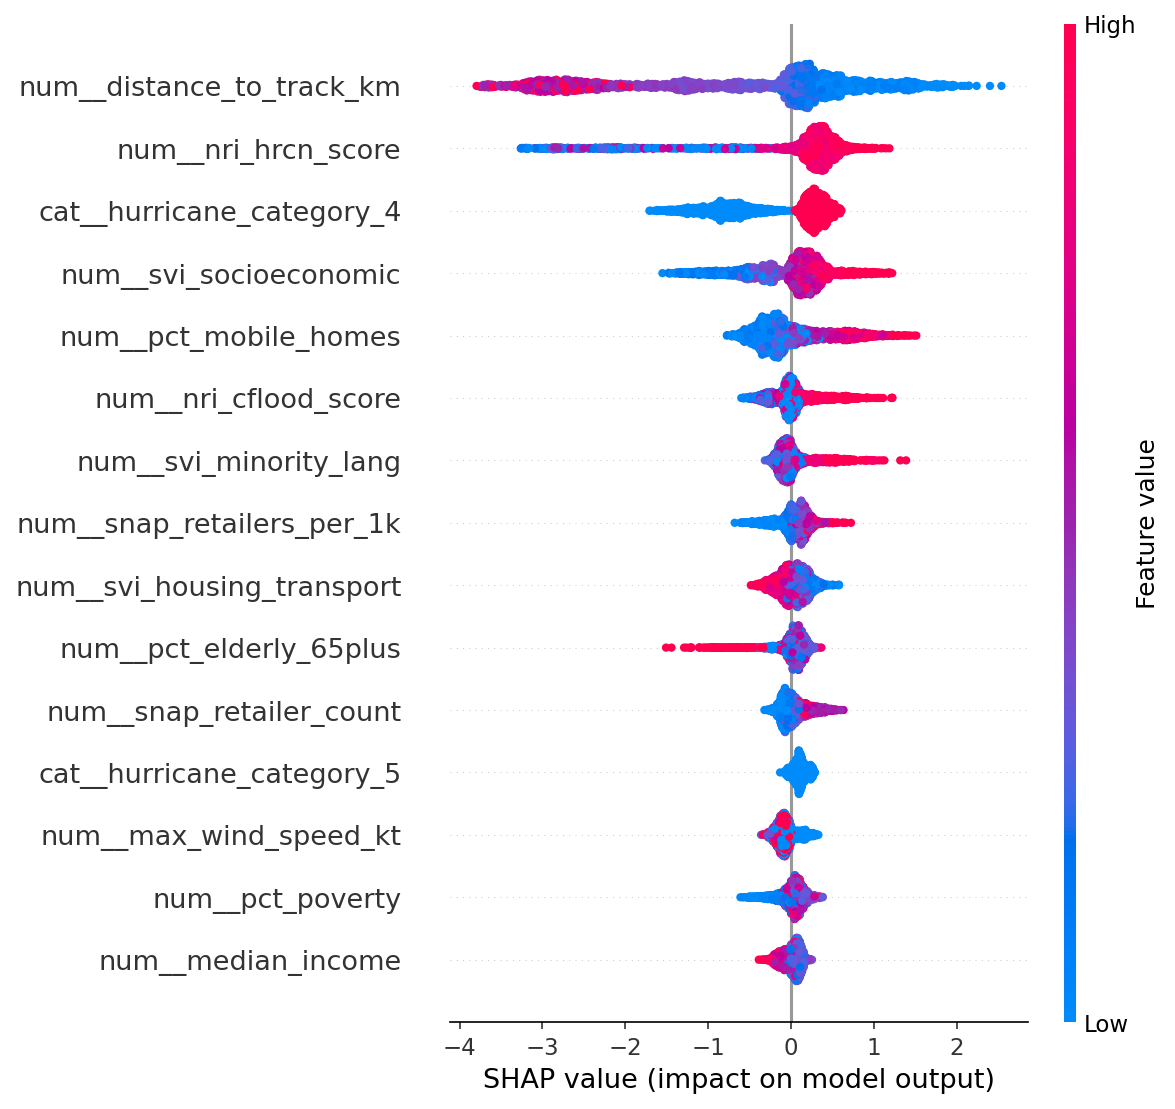
\includegraphics[width=0.95\columnwidth]{outputs/shap_beeswarm_severe.png}
\caption{SHAP beeswarm plot for the Severe damage class (XGBoost,
TEST set). Each point is one ZIP $\times$ hurricane observation.
Red = high feature value; blue = low feature value.
Storm proximity (\texttt{distance\_to\_track\_km}) and FEMA NRI
hurricane hazard score (\texttt{nri\_hrcn\_score}) are the
dominant predictors; social vulnerability features (SVI themes)
and food-access density (\texttt{snap\_retailers\_per\_1k})
contribute substantially.}
\label{fig:shap}
\end{figure}

The dominance of storm-geometry features (distance, category,
wind speed) is expected. Of greater humanitarian relevance is
the strong contribution of \texttt{svi\_socioeconomic} and
\texttt{pct\_mobile\_homes}: communities with lower incomes and
higher mobile-home prevalence are more likely to be classified
Severe at equivalent storm exposure, consistent with the
literature on structural vulnerability \cite{cutter_svi}.
The appearance of \texttt{snap\_retailers\_per\_1k} in the top
10 confirms that food-access geography independently informs
damage severity prediction beyond purely demographic signals.

\subsection{Priority Index Validation}

To validate the FRPI, we compare the top-50 and bottom-50
priority ZIP codes across the five TEST hurricanes:
\begin{itemize}
    \item \textbf{100\%} of top-50 ZIPs are classified as food
    deserts (vs.\ 0\% of bottom-50).
    \item Top-50 ZIPs rank in the \textbf{76th percentile}
    of national social vulnerability.
    \item Top-50 ZIPs experience \textbf{43$\times$} the actual
    FEMA-verified damage per 1,000 residents compared to the
    bottom-50.
\end{itemize}

The 43$\times$ damage ratio, measured against ground-truth FEMA
inspection data withheld from the model, provides strong evidence
that the FRPI captures operationally meaningful variation in
both physical damage and food-access vulnerability.

\subsection{IHP Registration Validation}

FEMA Individual Household Program (IHP) registration counts
are used as an independent validation signal. A Pearson
correlation $r > 0.85$ between per-ZIP FEMA inspector-verified
counts and IHP registration counts confirms that both measures
proxy the same underlying damage signal, supporting the use of
FEMA Housing Assistance data as the primary target.

% ============================================================
\section{Discussion}

\subsection{Operational Deployment}
The FRPI framework is designed to operate in \textit{pre-landfall}
mode: given storm track forecasts from the National Hurricane
Center and pre-computed community vulnerability scores, the model
produces ZIP-code priority rankings within minutes of a storm's
projected path becoming available. This positions relief
organizations to act during the critical 24--48 hour window
before landfall---when pre-positioning of food, water, and
personnel is still logistically feasible---rather than waiting
for post-event inspection data that arrives days too late.
The Streamlit dashboard
exposes five controls---hurricane selector, minimum priority
threshold, top-$N$ display, food-desert filter, and high-SVI
filter---sufficient for a logistics coordinator to generate
targeted resource allocation lists without requiring any ML
expertise. Per-ZIP SHAP waterfalls
explain each prediction in terms of the underlying features,
supporting accountability requirements in federally-funded
relief programs.

\subsection{Limitations}

\textbf{Temporal Coverage:} ACS 5-year estimates (2021 vintage)
are held static across all 14 hurricanes; ZIP-code demographic
conditions in 2016--2018 may differ from the 2021 snapshot.

\textbf{Regression Generalization:} Regression $R^2$ is negative
for Ida and Idalia, reflecting that diffuse inland flooding
events are qualitatively different from the coastal-track
pattern the model predominantly learns. The classifier is more
robust because its ordinal bins tolerate continuous prediction error.

\textbf{Food Atlas Vintage:} USDA Food Access Research Atlas
data from 2019 may not reflect food access conditions during
2021--2024 storms, particularly given the COVID-19-driven
expansion of SNAP and changes in supermarket footprints.

\textbf{ZIP-Code Aggregation:} ZIP codes are large and
heterogeneous; block-group or census-tract predictions would
offer finer targeting but require retraining on matched FEMA data.

\textbf{Class Imbalance:} Despite SMOTE oversampling,
the Low class dominates the training distribution, suppressing
Medium-class performance. More aggressive class-weighting
strategies merit exploration.

\subsection{Future Work}
Future directions include: (1) integrating real-time
precipitation and soil saturation data to improve
regression on inland flooding events; (2) extending the
framework to non-hurricane disasters (tornadoes, wildfires)
where food-access disruption follows different spatial
patterns; (3) replacing ZIP-code aggregation with tract-level
predictions using the full NRI hazard score granularity;
(4) deploying a live model update loop that ingests FEMA
inspection data as it arrives and re-ranks priority ZIP codes
within 24 hours of landfall.

% ============================================================
\section{Conclusion}

We presented an equitable, pre-landfall food relief
prioritization framework evaluated on 14 Atlantic hurricanes
spanning nearly a decade. The multi-source analytic base table,
hurricane-grouped temporal split, and FRPI design represent
a methodologically sound approach to a high-stakes humanitarian
resource allocation problem. The XGBoost classifier achieves
macro ROC-AUC 0.78 and Severe-class recall 0.82 on five
completely unseen hurricanes, and the FRPI correctly ranks
the 100\% food-desert, high-vulnerability ZIP codes as
highest priority---validating that the index captures genuine
operational need rather than statistical artifact.
Code, data pipeline, and dashboard are available at
\url{https://github.com/aneessaheba/hurricane-food-relief-ml}.
Most critically, the equity audit confirms that predictive
accuracy is \textit{highest} for the most socially vulnerable
communities. In a humanitarian deployment context, this is the
right direction: the framework does not merely avoid harming
underserved communities---it works \textit{better} for them,
making it suitable for operationalization by relief organizations
where equitable resource allocation is both a moral imperative
and a practical necessity.

% ============================================================
\section*{Acknowledgment}
The authors thank San Jos\'{e} State University for providing
the computational and institutional resources that supported
this research. The authors also thank the OpenFEMA program,
the U.S. Census Bureau ACS program, the CDC/ATSDR, and the
USDA Economic Research Service for making the underlying
datasets publicly available.

% ============================================================
\bibliographystyle{IEEEtran}
\begin{thebibliography}{00}

\bibitem{noaa_billion_dollar}
NOAA National Centers for Environmental Information (NCEI),
``U.S. Billion-Dollar Weather and Climate Disasters,''
\textit{NOAA NCEI}, 2024.
[Online]. Available: \url{https://www.ncei.noaa.gov/access/billions/}

\bibitem{coleman_jensen_food}
A. Coleman-Jensen, M. P. Rabbitt, C. A. Gregory, and A. Singh,
``Household Food Security in the United States in 2022,''
U.S. Department of Agriculture, Economic Research Report
No. ERR-325, 2023.

\bibitem{horney_food_disaster}
J. Horney, M. Nguyen, D. Salvesen, C. Tomasco, and P. Berke,
``Assessing the Relationship Between Hazard Mitigation Plan
Quality and Rural Status in a Sample of 57 Counties from
3 States in the U.S.,''
\textit{International Journal of Environmental Research and
Public Health}, vol. 14, no. 2, p. 212, 2017.

\bibitem{mayer_food_disaster}
B. Mayer, E. Running, and R. Bergstresser,
``Disasters, Civil Society Organizations, and Challenges of
Food Security,''
\textit{Disasters}, vol. 39, no. 4, pp. 717--739, 2015.

\bibitem{fema_response_timeline}
Federal Emergency Management Agency,
``Individual Assistance Program and Policy Guide,''
FEMA, Washington, DC, FP-104-009-03, 2021.

\bibitem{logistics_routing}
L. \"{O}zdamar, E. Ekinci, and B. K\"{u}\c{c}\"{u}kyazici,
``Emergency Logistics Planning in Natural Disasters,''
\textit{Annals of Operations Research},
vol. 129, no. 1--4, pp. 217--245, 2004.

\bibitem{shelter_allocation}
A. Anaya-Arenas, J. Renaud, and A. Ruiz,
``Relief distribution networks: a systematic review,''
\textit{Annals of Operations Research},
vol. 223, no. 1, pp. 53--79, 2014.

\bibitem{imran_social_media}
M. Imran, C. Castillo, F. Diaz, and S. Vieweg,
``Processing Social Media Messages in Mass Emergency: A Survey,''
\textit{ACM Computing Surveys}, vol. 47, no. 4, pp. 1--38, 2015.

\bibitem{hurricane_damage_models}
R. Merz, B. Kreibich, R. Schwarze, and A. Thieken,
``Review article: Assessment of economic flood damage,''
\textit{Natural Hazards and Earth System Sciences},
vol. 10, no. 8, pp. 1697--1724, 2010.

\bibitem{wang_disaster_logistics}
S. Wang, J. Watada, and W. Pedrycz,
``Recourse-Based Facility-Location Problems in Fuzzy Environments,''
\textit{IEEE Trans. Industrial Informatics}, vol. 6, no. 2,
pp. 196--208, 2010.

\bibitem{nateghi_power_outage}
R. Nateghi, S. D. Guikema, and S. M. Quiring,
``Power Outage Estimation for Tropical Cyclones: Improved
Accuracy with Simpler Models,''
\textit{Risk Analysis}, vol. 34, no. 6, pp. 1069--1078, 2014.

\bibitem{chakraborty_harvey}
J. Chakraborty, G. A. Collins, and M. Grineski,
``Exploring the Environmental Justice Implications of Hurricane
Harvey Flooding in Greater Houston, Texas,''
\textit{American Journal of Public Health},
vol. 109, no. 2, pp. 244--250, 2019.

\bibitem{usda_food_atlas}
U.S. Department of Agriculture, Economic Research Service,
``Food Access Research Atlas,'' 2019.
[Online]. Available:
\url{https://www.ers.usda.gov/data-products/food-access-research-atlas/}

\bibitem{flanagan_svi}
B. E. Flanagan, E. W. Gregory, E. J. Hallisey, J. L. Heitgerd,
and B. Lewis,
``A Social Vulnerability Index for Disaster Management,''
\textit{Journal of Homeland Security and Emergency Management},
vol. 8, no. 1, 2011.

\bibitem{cutter_svi}
S. L. Cutter, B. J. Boruff, and W. L. Shirley,
``Social Vulnerability to Environmental Hazards,''
\textit{Social Science Quarterly},
vol. 84, no. 2, pp. 242--261, 2003.

\bibitem{mehrabi_fairness}
N. Mehrabi, F. Morstatter, N. Saxena, K. Lerman, and A. Galstyan,
``A Survey on Bias and Fairness in Machine Learning,''
\textit{ACM Computing Surveys},
vol. 54, no. 6, pp. 1--35, 2021.

\bibitem{bird_fairlearn}
S. Bird, M. Dud\'{i}k, R. Edgar, B. Horn, R. Lutz, V. Milan,
M. Sameki, H. Wallach, and K. Walker,
``Fairlearn: A Toolkit for Assessing and Improving Fairness in
AI,'' Microsoft Research, Tech. Rep. MSR-TR-2020-32, 2020.

\bibitem{lundberg_shap}
S. M. Lundberg and S.-I. Lee,
``A Unified Approach to Interpreting Model Predictions,''
in \textit{Proc. 31st Conf. Neural Information Processing
Systems (NeurIPS)}, Long Beach, CA, 2017, pp. 4765--4774.

\bibitem{chawla_smote}
N. V. Chawla, K. W. Bowyer, L. O. Hall, and W. P. Kegelmeyer,
``SMOTE: Synthetic Minority Over-Sampling Technique,''
\textit{Journal of Artificial Intelligence Research},
vol. 16, pp. 321--357, 2002.

\bibitem{chen_xgboost}
T. Chen and C. Guestrin,
``XGBoost: A Scalable Tree Boosting System,''
in \textit{Proc. 22nd ACM SIGKDD Int. Conf. Knowledge Discovery
and Data Mining}, San Francisco, CA, 2016, pp. 785--794.

\bibitem{optuna}
T. Akiba, S. Sano, T. Yanase, T. Ohta, and M. Koyama,
``Optuna: A Next-Generation Hyperparameter Optimization
Framework,'' in \textit{Proc. 25th ACM SIGKDD Int. Conf.
Knowledge Discovery and Data Mining}, 2019, pp. 2623--2631.

\bibitem{pedregosa_sklearn}
F. Pedregosa, G. Varoquaux, A. Gramfort, \textit{et al.},
``Scikit-learn: Machine Learning in Python,''
\textit{Journal of Machine Learning Research},
vol. 12, pp. 2825--2830, 2011.

\bibitem{knapp_ibtracs}
K. R. Knapp, M. C. Kruk, D. H. Levinson, H. J. Diamond,
and C. J. Neumann,
``The International Best Track Archive for Climate Stewardship
(IBTrACS): Unifying Tropical Cyclone Data,''
\textit{Bulletin of the American Meteorological Society},
vol. 91, no. 3, pp. 363--376, 2010.

\end{thebibliography}

\end{document}
